\documentclass[border=3pt,tikz]{standalone}
\usepackage{amsmath}
\usetikzlibrary{arrows.meta}
\usetikzlibrary{calc}
\begin{document}
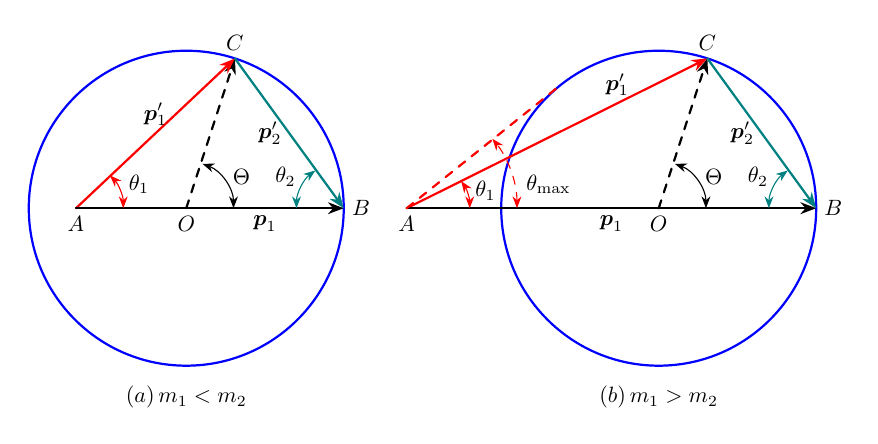
\begin{tikzpicture}[line cap=round, scale = 2]

    \coordinate (A) at (-0.7, 0);
    \coordinate (B) at (1.0, 0);
    \coordinate (C) at (0.309, 0.951);
    
    \draw[fill=none, blue, thick](0,0) circle (1);
    \draw[dashed, thick,  -{Stealth[length=2mm]}] (0, 0) node [below, scale=0.8] {$O$} -- (C) node [above, scale=0.8] {$C$};
    \draw[thick, red,  -{Stealth[length=2mm]}] (A) node [below, black, scale=0.8] {$A$} -- (C);
    \draw[thick, teal,  -{Stealth[length=2mm]}] (C) -- (B) node [right, black, scale=0.8] {$B$} ;
    \draw[thick, black,-{Stealth[length=2mm]}] (A) -- (B);
    \node[below, scale=0.8] at (0.5, 0) {$\boldsymbol{p}_1$};
    
    \draw [{Stealth[length=1.5mm]}-{Stealth[length=1.5mm]}] (0.3,0.0) arc (0:70:0.3);
    \node [scale=0.8] at (0.35, 0.2) {$\Theta$};
    
    \draw [teal, {Stealth[length=1.5mm]}-{Stealth[length=1.5mm]}] (0.7,0.0) arc (180:127:0.3);
    \node [scale=0.8] at (0.63, 0.2) {$\theta_2$};
    
    \draw [red, {Stealth[length=1.5mm]}-{Stealth[length=1.5mm]}] (-0.4,0.0) arc (0:44:0.3);
    \node [scale=0.8] at (-0.3, 0.15) {$\theta_1$};
    
    \node[above,scale=0.8] at ($0.5*(A) + 0.5*(C)$ ){$\boldsymbol{p}'_1$};
    \node[left,scale=0.8] at ($0.5*(B) + 0.5*(C)$ ){$\boldsymbol{p}'_2$};
    \node[scale=0.8] at (0.0, -1.2) {$(a)\, m_1<m_2$};
    
    %\node [below, scale=0.8] at ($0.5*(A)$) {$\boldsymbol{p}_A$};
    %\node [below, scale=0.8] at ($0.5*(B)$) {$\boldsymbol{p}_B$};
    
    
    \begin{scope}[shift={(3,0)}]
    \coordinate (A) at (-1.6, 0);
    \coordinate (B) at (1.0, 0);
    \coordinate (C) at (0.309, 0.951);
    
    \draw[fill=none, blue, thick](0,0) circle (1);
    \draw[dashed, thick,  -{Stealth[length=2mm]}] (0, 0) node [below, scale=0.8] {$O$} -- (C) node [above, scale=0.8] {$C$};
    \draw[thick, red,  -{Stealth[length=2mm]}] (A) node [below, black, scale=0.8] {$A$} -- (C);
    \draw[thick, teal,  -{Stealth[length=2mm]}] (C) -- (B) node [right, black, scale=0.8] {$B$} ;
    \draw[thick, black,-{Stealth[length=2mm]}] (A) -- (B);
    \node[below, scale=0.8] at (-0.3, 0) {$\boldsymbol{p}_1$};
    
    \draw [{Stealth[length=1.5mm]}-{Stealth[length=1.5mm]}] (0.3,0.0) arc (0:70:0.3);
    \node [scale=0.8] at (0.35, 0.2) {$\Theta$};
    
    \draw [teal, {Stealth[length=1.5mm]}-{Stealth[length=1.5mm]}] (0.7,0.0) arc (180:127:0.3);
    \node [scale=0.8] at (0.63, 0.2) {$\theta_2$};
    
    \draw [red, {Stealth[length=1.5mm]}-{Stealth[length=1.5mm]}] (-1.2,0.0) arc (0:35:0.3);
    \node [scale=0.8] at (-1.1, 0.11) {$\theta_1$};
    \draw [thick, red, dashed] (A) -- (-0.625, 0.7806);
    \draw [red, dashed, {Stealth[length=1.5mm]}-{Stealth[length=1.5mm]}] (-0.9,0.0) arc (0:39:0.7);
    \node [scale=0.8] at (-0.70, 0.15) {$\theta_{\textrm{max}}$};
    
    \node[above,scale=0.8] at ($0.3*(A) + 0.7*(C)$ ){$\boldsymbol{p}'_1$};
    \node[left,scale=0.8] at ($0.5*(B) + 0.5*(C)$ ){$\boldsymbol{p}'_2$};
    
    \node[scale=0.8] at (0.0, -1.2) {$(b)\, m_1>m_2$};
    \end{scope}
    
    
    \end{tikzpicture}
\end{document}